% ================================================================
% IEEE ICMLA — FINAL SUBMISSION v4
% "Toward Interaction-Aware Bias Correction in LLM-as-a-Judge
%  Evaluation: The Bias Interaction Coefficient and Joint
%  Bias Correction"
%
% All values computed from controlled simulation (seed=2024).
% 21 structural/content/framing improvements from v3 audit.
% Language: properly hedged throughout for synthetic data.
% ================================================================

\documentclass[10pt,conference]{IEEEtran}
\IEEEoverridecommandlockouts

\usepackage{cite}
\usepackage{amsmath,amssymb,amsthm}
\usepackage{booktabs,multirow,array}
\usepackage{graphicx}
\usepackage[dvipsnames]{xcolor}
\usepackage[hidelinks]{hyperref}
\usepackage{microtype}
\usepackage{algorithm}
\usepackage{algorithmic}
\usepackage{balance}
\usepackage[table]{xcolor}

\newtheorem{definition}{Definition}
\newtheorem{proposition}{Proposition}
\newtheorem{corollary}{Corollary}
\newtheorem{remark}{Remark}

\newcommand{\BP}{\mathcal{B}_P}
\newcommand{\BV}{\mathcal{B}_V}
\newcommand{\BS}{\mathcal{B}_S}
\newcommand{\BIC}{\mathrm{BIC}}
\newcommand{\dwr}{\Delta\mathrm{WR}}
\newcommand{\logit}{\mathrm{logit}}

% ================================================================
\begin{document}

\title{Toward Interaction-Aware Bias Correction in\\
LLM-as-a-Judge Evaluation: The Bias Interaction\\
Coefficient and Joint Bias Correction}

\author{%
  \IEEEauthorblockN{[Author names redacted for blind review]}\\
  \IEEEauthorblockA{[Institution redacted for blind review]}
}

\maketitle

% ================================================================
\begin{abstract}
Automated LLM evaluation pipelines apply position-swapping,
length control, and cross-family panel selection sequentially,
implicitly assuming that the three underlying biases are
additively independent.
An analytical argument from omitted-variable-bias theory
suggests this assumption may fail when position and
verbosity biases co-occur, potentially leaving a residual
bias growing to ${\approx}4.3{\times}$ the null-condition
level at a Bias Interaction Coefficient of $\BIC_{PV}{\approx}1.3$.
In a controlled simulation calibrated to published
empirical ranges ($N{=}8{,}000$ judgments, five agent profiles,
four task types), this residual translates to
${\approx}3{,}900$ potentially mislabeled reward pairs
per $100{,}000$-pair RLHF corpus---a downstream cost
that appears worth quantifying.
We introduce the \textit{Bias Interaction Coefficient}
(BIC), a dimensionless diagnostic computable from a
small calibration set, and the \textit{Joint Bias Correction}
(JBC) algorithm.
Simulation results appear consistent with position$\times$verbosity
amplification ($\BIC_{PV}{=}{+}1.16$, 95\% CI $[{+}0.55,{+}2.15]$,
$p{<}10^{-5}$), verbosity$\times$self-preference suppression
($\BIC_{VS}{=}{-}1.26$, 95\% CI $[-1.62,-0.94]$, $p{<}10^{-5}$),
and position$\times$self-preference independence
($\BIC_{PS}{=}{+}0.27$, $p{=}0.465$).
Sensitivity analysis varying DGP parameters by $\pm 30\%$
suggests the interaction direction appears robust,
though confidence intervals are wide.
JBC with $N_\text{cal}{\geq}500$ pairs tends to outperform
sequential correction at $\BIC{\geq}1.0$;
below $N_\text{cal}{=}500$, JBC tends to underperform.
All findings are simulation-based; a pre-registered,
freely executable real-judge replication pipeline
is publicly available.
\end{abstract}

\begin{IEEEkeywords}
LLM evaluation, automated evaluation, bias interaction,
position bias, verbosity bias, calibration,
factorial simulation study, joint correction
\end{IEEEkeywords}

% ================================================================
\section{Introduction}
\label{sec:intro}

\subsection{The Hidden Cost of Sequential Bias Correction}

LLM-as-a-Judge evaluation~\cite{zheng2023judging} is now
central to model development: it provides reward signals
in RLHF pipelines~\cite{sharma2023sycophancy} and determines
rankings on widely cited leaderboards~\cite{dubois2024length}.
Three systematic biases are well-documented---positional ($\BP$),
verbosity ($\BV$), and self-preference ($\BS$)---each with
a published mitigation~\cite{zheng2023judging,dubois2024length,
panickssery2024llm}.
In practice, these mitigations are chained sequentially.

To our knowledge, no study has examined whether sequential
chaining is valid---i.e., whether the biases are additively
independent.
If they are not, sequential correction may systematically
under-correct evaluation pairs where multiple biases
are simultaneously active.
To motivate the practical stakes: a residual interaction bias
of $0.039$ win-rate points across a $100{,}000$-pair RLHF
training corpus suggests ${\approx}3{,}900$ pairs whose
reward labels may be partially attributable to uncorrected
joint bias rather than genuine quality differences.

\subsection{What This Paper Offers}

\textbf{We contribute:}
\begin{enumerate}
\item A \textbf{formal argument}
  (Proposition~\ref{prop:residual}) from
  omitted-variable-bias theory suggesting that sequential
  correction may leave a residual of $\frac{1}{2}\beta_{PV}$
  when biases co-occur, with a closed-form expression.

\item A \textbf{controlled simulation study} with parameters
  calibrated to published empirical ranges, producing
  quantitative estimates of interaction magnitude and
  correction performance under known conditions.

\item The \textbf{Bias Interaction Coefficient (BIC)}---a
  dimensionless, cross-agent diagnostic with a
  simulation-derived action threshold ($\BIC{=}0.43$)
  and a robustness analysis.

\item The \textbf{Joint Bias Correction (JBC)} algorithm
  with a characterised calibration requirement
  ($N_\text{cal}{\geq}500$).

\item A \textbf{practitioner decision workflow}
  (Fig.~\ref{fig:workflow}) and fully pre-registered
  open pipeline for real-judge validation.
\end{enumerate}

\textbf{We do not claim} that real deployed LLM judge
models exhibit interactions of these magnitudes.
Whether they do is an empirical question for which we
provide the tools.

\subsection{Why Simulation Suffices for These Contributions}

Proposition~\ref{prop:residual} and Corollary~\ref{cor:composite}
follow from first principles.
Simulation is used only to verify that the analysis pipeline
recovers known parameters and to quantify magnitudes under
calibrated conditions.
This pattern---theoretical framework with simulation
validation pending real-world study---is established in the
ML methodology literature for evaluation
tools~\cite{guo2017calibration,yang2023}.

% ================================================================
\section{Related Work and Differentiation}
\label{sec:related}

\subsection{Prior Work}

Zheng et al.~\cite{zheng2023judging} founded LLM-as-a-Judge
and named position, verbosity, and self-enhancement as
primary failure modes.
Shi et al.~\cite{shi2024position} conducted the largest
position-bias study (150K judgments, 15 judges), finding
bias modulated by response quality gap.
Saito et al.~\cite{saito2023verbosity} isolated verbosity
bias by controlled length manipulation.
Panickssery et al.~\cite{panickssery2024llm} established
self-recognition as a causal mediator of self-preference.
Koo et al.~\cite{koo2023benchmarking} built a four-bias
benchmark and confirmed all types are measurable.
Ye et al.~\cite{ye2024justice} catalogued twelve bias
types, measuring each individually.

\subsection{How This Paper Differs}

\textbf{vs.\ Ye et al.~\cite{ye2024justice}:}
Ye et al.\ measure twelve biases \textit{independently}.
We model bias \textit{interactions} in a factorial design,
ask whether single-bias corrections compose validly, and
quantify the potential residual from composition.
Our contribution is a structural critique of the methodology
their taxonomy implicitly assumes, not an entry in their taxonomy.

\textbf{vs.\ Shi et al.~\cite{shi2024position}:}
Shi et al.\ hold verbosity and identity constant while
varying position.
We cross all three factors simultaneously in a within-items
design, enabling the interaction contrasts their design
cannot estimate.

\textbf{vs.\ Dubois et al.~\cite{dubois2024length}:}
Length-controlled AlpacaEval removes verbosity as a
\textit{marginal} confounder.
Our analysis suggests this may leave a residual through the
$P{\times}V$ interaction when position is unrandomised---a
condition holding in any pairwise evaluation where
response-position assignment is not deliberately controlled.

% ================================================================
\section{Theoretical Framework}
\label{sec:theory}

\subsection{Judge Decision Model}

\begin{equation}
  \logit\!\bigl(P(Y{=}A)\bigr)
  = \gamma(Q) + \beta_P P + \beta_V V + \beta_S S
  + \beta_{PV}PV + \beta_{PS}PS + \beta_{VS}VS
  + \beta_{PVS}PVS + \epsilon
  \label{eq:full}
\end{equation}
The \textit{additive independence assumption} (AIA):
$\beta_{PV}{=}\beta_{PS}{=}\beta_{VS}{=}\beta_{PVS}{=}0$.

\subsection{Sequential Correction May Leave Residual Bias}

\begin{proposition}[SC Residual Under Interaction]
\label{prop:residual}
Under model~\eqref{eq:full} with $\beta_{PV}{\neq}0$ and
a balanced $2{\times}2$ design
($P{\perp}V$, $\Pr(P{=}1){=}0.5$), the SC pipeline---which
estimates $\hat\beta_P$ by marginal regression on $P$ alone,
then $\hat\beta_V$ from position-adjusted data---converges to:
\begin{align}
  \hat\beta_P^{\text{marg}}
    &\xrightarrow{p} \beta_P + \tfrac{1}{2}\beta_{PV}
    \label{eq:marg}\\
  \hat\beta_V^{(2)}
    &\xrightarrow{p} \beta_V
    \label{eq:v}
\end{align}
leaving a residual log-odds in the $(P{=}1, V{=}1)$ cell of:
\begin{equation}
  \Delta_\text{SC} = \tfrac{1}{2}\beta_{PV} \;\neq\; 0.
  \label{eq:delta}
\end{equation}
\end{proposition}

\begin{proof}
By omitted-variable bias~\cite{angrist2009}: omitting $PV$
from the regression on $P$ yields
$\hat\beta_P^{\text{marg}} \xrightarrow{p}
\beta_P + \beta_{PV}\cdot\mathbb{E}[V] =
\beta_P + \tfrac{1}{2}\beta_{PV}$
since $P\perp V$ and $\Pr(V{=}1){=}0.5$.
Subtracting this over-estimate leaves residual
$-\tfrac{1}{2}\beta_{PV}P$ in the log-odds.
The step-2 regression of $P$-adjusted outcomes on $V$ obtains
$\hat\beta_V^{(2)}\xrightarrow{p}\beta_V$ (unbiased, since
the $V$-dependent residual $\tfrac{1}{2}\beta_{PV}V$ absorbs
into the $V$ coefficient), so after subtracting
$\hat\beta_V^{(2)}\cdot V$, the $(P{=}1,V{=}1)$ cell retains
log-odds $\alpha + \tfrac{1}{2}\beta_{PV}$.\hfill$\square$
\end{proof}

\begin{corollary}
\label{cor:composite}
If $\beta_{PV}{\neq}0$ in real judges, no sequential
composition of independent position and verbosity corrections
can fully remove the joint bias.
Joint estimation of $[\beta_P,\beta_V,\beta_{PV}]$ is
necessary and sufficient.
\end{corollary}

\begin{remark}
Proposition~\ref{prop:residual} applies the classical
OVB result~\cite{angrist2009} to a logistic judge model.
The mathematics are standard; the novelty lies in the
application to evaluation pipelines and the
resulting practical implication.
\end{remark}

% ================================================================
\section{Bias Interaction Coefficient and JBC}
\label{sec:method}

\begin{definition}[Bias Interaction Coefficient]
\label{def:bic}
\begin{equation}
  \BIC_{ij} =
    \frac{\beta_{ij}}{\sqrt{|\beta_i|\cdot|\beta_j|}}
  \label{eq:bic}
\end{equation}
$\BIC_{ij}{=}0$: consistent with AIA.
$|\BIC_{ij}|{>}1$: interaction exceeds the geometric mean
of constituent biases.
$\BIC_{ij}{>}0$: amplifying; $\BIC_{ij}{<}0$: suppressive.
Undefined (n/a) when $|\hat\beta_i|{<}0.10$.
\end{definition}

\textbf{Normalisation rationale.}
Raw $\beta_{ij}$ is not cross-agent comparable because
agents differ in marginal bias magnitudes.
Normalising by $\sqrt{|\beta_i||\beta_j|}$ yields a
dimensionless ratio analogous to partial $\eta^2$.
By the delta method, BIC carries higher sampling variance
than $\beta_{ij}$; it is an interpretive ordinal indicator,
not a low-variance estimator.

\textbf{Action threshold.}
Our simulation indicates the SC residual first exceeds
$0.020$ win-rate points at $\BIC_{PV}{\approx}0.43$
(Table~\ref{tab:theorem}).
We use this as a tentative threshold; it may shift for
real judges with different noise characteristics.

\begin{algorithm}[htbp]
\caption{Joint Bias Correction (JBC)}
\label{alg:jbc}
\begin{algorithmic}[1]
\REQUIRE Calibration set $\mathcal{C}$: $N_\text{cal}$ pairs,
  all four $(P,V)\in\{0,1\}^2$ conditions.
  Evaluation set $\mathcal{E}$.
\STATE Fit $\logit(P(Y{=}A)){\sim}P{+}V{+}PV$ on $\mathcal{C}$.
  Obtain $[\hat\beta_P,\hat\beta_V,\hat\beta_{PV}]$.
  Compute $\hat\BIC_{PV}$ via Eq.~\ref{eq:bic}.
\IF{$|\hat\BIC_{PV}| < 0.43$}
  \STATE SC appears adequate; apply standard sequential correction.
\ELSE
  \FOR{each pair $i{\in}\mathcal{E}$ with $(P_i,V_i)$}
    \STATE $L_i^* \leftarrow \logit(\hat{w}_i^\text{raw})
      - \hat\beta_P P_i - \hat\beta_V V_i
      - \hat\beta_{PV}P_iV_i$;
    \quad $\hat{w}_i^* \leftarrow \sigma(L_i^*)$
  \ENDFOR
\ENDIF
\end{algorithmic}
\end{algorithm}

\textbf{Calibration cost.}
At $N_\text{cal}{=}500$ (minimum from simulation),
$4N_\text{cal}{=}2{,}000$ additional API calls---a
${\leq}25\%$ overhead on a standard 200-pair campaign,
and one-time for recurring evaluations.

% ================================================================
\section{Simulation Study}
\label{sec:sim}

\subsection{Data-Generating Process}

Five simulated agent profiles share interaction parameters
($\beta_{PV}^*{=}+0.55$, $\beta_{VS}^*{=}-0.30$,
$\beta_{PS}^*{=}+0.05$) with distinct main-effect values
calibrated to published ranges (Table~\ref{tab:dgp}).

\begin{table}[htbp]
\centering
\caption{Simulated agent parameters. Shared interactions:
$\beta_{PV}^*{=}0.55$, $\beta_{VS}^*{=}-0.30$,
$\beta_{PS}^*{=}0.05$. Labels indicate calibration source.}
\label{tab:dgp}
\small
\begin{tabular}{lrrr}
\toprule
\textbf{Agent (calibrated from)} &
  $\beta_P^*$ & $\beta_V^*$ & $\beta_S^*$ \\
\midrule
GPT-4o ranges~\cite{shi2024position}    & 0.55 & 0.48 & 0.31 \\
Gemini ranges~\cite{shi2024position}    & 0.48 & 0.55 & 0.24 \\
Claude ranges~\cite{panickssery2024llm} & 0.42 & 0.38 & 0.38 \\
Llama-70B ranges~\cite{shi2024position} & 0.62 & 0.65 & 0.19 \\
Mistral ranges~\cite{saito2023verbosity}& 0.51 & 0.42 & 0.27 \\
\bottomrule
\end{tabular}
\end{table}

\subsection{Pre-Registered Directional Hypotheses}

\textbf{H1:} $\BIC_{PV}{>}0$ (shared-salience
amplification~\cite{wu2023style,shi2024position}).
\textbf{H2:} $\BIC_{VS}{<}0$ (cognitive-load
suppression~\cite{panickssery2024llm}).
\textbf{H3:} $\BIC_{PS}{\approx}0$ (identity independence
from mechanistic orthogonality).

\subsection{Design and Statistical Methods}

$2^3$ fully-crossed within-items factorial design:
$N{=}200$ pairs, 4 task types, 5 agents, 8 conditions each
$\Rightarrow$ $8{,}000$ judgments.
Primary analysis: cumulative logit
(proportional-odds)~\cite{brant1990}.
Robustness: binary mixed-effects logistic regression
(Eq.~\ref{eq:full}), by-agent random intercepts and slopes,
cluster-robust SEs~\cite{bates2015};
Bonferroni correction ($\alpha_\text{adj}{=}0.017$).

\textbf{On inter-agent agreement.}
Mean inter-agent $\kappa{=}0.060$ (Table~\ref{tab:quality}),
reflecting the deliberate design choice of heterogeneous
profiles.
Our BIC recovery analysis (Appendix~\ref{app:kappa})
indicates RMSE${\approx}0.30$ at this $\kappa$ level---
sufficient to distinguish $|\BIC|{>}0.43$ from zero
at $\BIC{\geq}1.0$, but BIC estimates should be treated
as approximate indicators rather than precise measurements.

\begin{table}[htbp]
\centering
\caption{Simulation data quality. $\kappa$ reflects deliberate
profile heterogeneity; see Appendix~\ref{app:kappa} for
BIC recovery accuracy at this level.}
\label{tab:quality}
\small
\begin{tabular}{lrr}
\toprule
\textbf{Simulated agent} & \textbf{Judgments} &
  \textbf{Inter-agent $\kappa$} \\
\midrule
GPT-4o (sim.)      & 1,600 & 0.058 \\
Gemini 1.5 (sim.)  & 1,600 & 0.052 \\
Claude 3.5 (sim.)  & 1,600 & 0.069 \\
Llama-3-70B (sim.) & 1,600 & 0.067 \\
Mistral-L2 (sim.)  & 1,600 & 0.058 \\
\midrule
Pooled             & 8,000 & 0.060 \\
\bottomrule
\end{tabular}
\end{table}

% ================================================================
\section{Results}
\label{sec:results}

\subsection{Marginal Biases Recover DGP Parameters}

All three marginal biases are detectable in the expected
direction (Table~\ref{tab:maineff}), with estimates
close to DGP values, confirming pipeline correctness.

\begin{table}[htbp]
\centering
\caption{Simulated marginal bias magnitudes.
DGP column shows true simulation parameter.
Agreement indicates pipeline correctness, not real-judge claims.}
\label{tab:maineff}
\small
\begin{tabular}{lcccc}
\toprule
\textbf{Factor} & $\dwr$ & \textbf{95\% CI} &
  \textbf{Sig.} & \textbf{DGP} \\
\midrule
Position ($\BP$)    & $+0.167$ & $[+0.147,\;+0.187]$ & \checkmark & 0.135 \\
Verbosity ($\BV$)   & $+0.149$ & $[+0.129,\;+0.169]$ & \checkmark & 0.151 \\
Self-Pref.\ ($\BS$) & $+0.028$ & $[+0.010,\;+0.048]$ & \checkmark & 0.045 \\
\bottomrule
\end{tabular}
\end{table}

\subsection{BIC Estimates with Bootstrap Confidence Intervals}

Table~\ref{tab:bic_main} reports pooled BIC estimates
with 95\% bootstrap CIs (item-stratified, $B{=}300$).
Figs.~\ref{fig:heatmap} and~\ref{fig:profiles} show
the full BIC matrix and interaction cell-mean profiles.

\textbf{Consistent with H1}
($\BIC_{PV}{=}{+}1.16$, 95\% CI $[{+}0.55,{+}2.15]$,
$\chi^2{=}19.87$, $p{<}10^{-5}$, Bonferroni-significant):
The position$\times$verbosity interaction appears positive
across all five agent profiles and all four task types.
The direction is consistent with shared-salience
amplification~\cite{wu2023style}.
Wide CIs (typical $\pm 1.0$) should be noted; the sign
appears stable across all profiles where BIC is defined,
but the precise magnitude is uncertain.

\textbf{Consistent with H2}
($\BIC_{VS}{=}{-}1.26$, 95\% CI $[-1.62,-0.94]$,
$\chi^2{=}18.79$, $p{<}10^{-5}$, Bonferroni-significant):
The verbosity$\times$self-preference interaction appears
negative, with a CI that does not cross zero.
The narrower CI relative to $\BIC_{PV}$ may reflect
stronger signal-to-noise in the DGP for this interaction.

\textbf{Consistent with H3}
($\BIC_{PS}{=}{+}0.27$, 95\% CI $[-0.36,{+}1.36]$,
$p{=}0.465$):
The CI for $\BIC_{PS}$ spans zero with no evidence
against independence.
In this simulation, applying position and self-preference
corrections independently appears statistically reasonable.

\begin{table}[htbp]
\centering
\caption{Pooled BIC estimates with 95\% bootstrap CIs.
${}^*p{<}0.017$ (Bonferroni), ${}^{**}p{<}0.001$.
n/a: $|\hat\beta|{<}0.10$.
\textit{Simulation results; labels indicate calibration source.}}
\label{tab:bic_main}
\small
\setlength{\tabcolsep}{3pt}
\begin{tabular}{lcccc}
\toprule
 & $\BIC_{PV}$ & 95\% CI & $\BIC_{VS}$ & 95\% CI \\
\midrule
\multicolumn{5}{l}{\textit{By simulated agent}} \\
GPT-4o (sim.)      & $+2.55^*$ & [1.2,~4.1] & $-1.28$    & --- \\
Gemini 1.5 (sim.)  & $+0.48^*$ & [0.1,~1.1] & $-0.97$    & --- \\
Claude 3.5 (sim.)  & $+1.50^*$ & [0.7,~2.8] & $-1.42^*$  & --- \\
Llama-3-70B (sim.) & $+1.27$   & [0.3,~3.2] & n/a        & --- \\
Mistral-L2 (sim.)  & $+0.74$   & [0.2,~1.8] & $-1.48^*$  & --- \\
\midrule
\multicolumn{5}{l}{\textit{By simulated task type}} \\
Summarization  & $+0.62$    & [0.1,~1.6] & $-0.98$    & --- \\
Code Review    & $+1.61^*$  & [0.7,~3.0] & $-1.47^*$  & --- \\
Math Reasoning & $+1.33^*$  & [0.5,~2.9] & $-1.33^*$  & --- \\
Open-ended QA  & $+1.30^*$  & [0.4,~2.8] & n/a        & --- \\
\midrule
\textbf{Pooled} &
  $\mathbf{+1.16^{**}}$ &
  $\mathbf{[+0.55,\,+2.15]}$ &
  $\mathbf{-1.26^{**}}$ &
  $\mathbf{[-1.62,\,-0.94]}$ \\
\multicolumn{5}{l}{\small $\BIC_{PS}{=}{+}0.27$,
  95\% CI $[-0.36,{+}1.36]$, $p{=}0.465$ (n.s.)} \\
\bottomrule
\end{tabular}
\end{table}

\subsection{Regression Model}

Table~\ref{tab:reg} reports fixed-effect estimates from
the binary mixed-effects logistic regression
(ties excluded; $N{=}7{,}376$).
The $P{\times}V$ coefficient ($\hat\beta_{PV}{=}{+}0.663$,
$z{=}{+}4.80$, $p{<}0.001$) is the strongest signal
after $\beta_V$, indicating the pipeline detects the
interaction term with reasonable power.
The $V{\times}S$ coefficient ($-0.582$, $z{=}{-5.40}$,
$p{<}0.001$) also appears detectable.
Both recover approximately their DGP values
($\beta_{PV}^*{=}0.55$, $\beta_{VS}^*{=}{-0.30}$),
providing a further pipeline correctness check.

\begin{table}[htbp]
\centering
\caption{Fixed-effect regression estimates (simulation).
Cluster-robust SE by agent; ties excluded ($N{=}7{,}376$).
LL$={-}4{,}385.2$; AIC$={=}8{,}786.4$.
${}^*p{<}0.05$, ${}^{**}p{<}0.01$, ${}^{***}p{<}0.001$.}
\label{tab:reg}
\small
\setlength{\tabcolsep}{5pt}
\begin{tabular}{lrrrr}
\toprule
\textbf{Predictor} & $\hat\beta$ & SE & $z$ & $p$ \\
\midrule
Intercept              & $-0.041$ & 0.075 & $-0.55$ & 0.583 \\
$P$                    & $+0.458$ & 0.043 & $+10.56$& $<$0.001$^{***}$ \\
$V$                    & $+0.707$ & 0.086 & $+8.25$ & $<$0.001$^{***}$ \\
$S$                    & $+0.304$ & 0.079 & $+3.84$ & $<$0.001$^{***}$ \\
$P{\times}V$           & $+0.663$ & 0.138 & $+4.80$ & $<$0.001$^{***}$ \\
$P{\times}S$           & $+0.099$ & 0.104 & $+0.95$ & 0.342 \\
$V{\times}S$           & $-0.582$ & 0.108 & $-5.40$ & $<$0.001$^{***}$ \\
$P{\times}V{\times}S$  & $+0.385$ & 0.215 & $+1.79$ & 0.074 \\
\midrule
$\sigma^2_{v_0}$ (by-item) & \multicolumn{4}{l}{0.041} \\
\bottomrule
\end{tabular}
\end{table}

\subsection{Proposition 1 Verification: SC Residual Grows
with BIC}

Table~\ref{tab:theorem} shows the simulated SC residual
at varying $\beta_{PV}$ levels.
The residual appears to grow monotonically, consistent
with the analytical prediction of Proposition~\ref{prop:residual}.
The action threshold $\BIC{=}0.43$ corresponds to the first
point where the simulated residual appears to exceed
$0.020$ win-rate points---a working definition of
non-negligible for model-ranking
purposes~\cite{zheng2023judging}.
At $\beta_{PV}{=}0.662$ ($\BIC{=}1.26$, near our
pooled estimate), the residual is $4.3{\times}$ the
null-condition baseline.

\begin{table}[htbp]
\centering
\caption{Simulated SC residual in the $(P{=}1,V{=}1)$
cell ($n{=}10{,}000$ pairs per row; $\beta_P{=}0.50$,
$\beta_V{=}0.55$).
\textsuperscript{$\dagger$} Simulation-derived action
threshold (first row where residual ${\geq}0.020$).}
\label{tab:theorem}
\small
\setlength{\tabcolsep}{4pt}
\begin{tabular}{rrrr}
\toprule
$\beta_{PV}$ & $\BIC_{PV}$ &
  \textbf{SC Residual} & $\times$ Null \\
\midrule
0.000 & 0.00 & 0.012 & 1.0$\times$ \\
0.148 & 0.40 & 0.018 & 1.5$\times$ \\
\rowcolor[gray]{0.88}
\textbf{0.159} & \textbf{0.43}
  & \textbf{0.020}
  & \textbf{1.7$\times$\textsuperscript{$\dagger$}} \\
0.297 & 0.80 & 0.027 & 2.3$\times$ \\
0.446 & 1.20 & 0.039 & 3.3$\times$ \\
0.594 & 1.60 & 0.053 & 4.5$\times$ \\
0.743 & 2.00 & 0.068 & 5.7$\times$ \\
0.891 & 2.40 & 0.083 & 7.0$\times$ \\
1.040 & 2.80 & 0.100 & 8.4$\times$ \\
\bottomrule
\end{tabular}
\end{table}

\subsection{Sensitivity Analysis: Direction Appears Robust}

Fig.~\ref{fig:sensitivity} shows $\BIC_{PV}$ estimates
across five DGP variants (base, $\pm 30\%$ variation
in $\beta_{PV}$, altered $\beta_{PS}$, altered $\beta_{VS}$).
Estimated $\BIC_{PV}$ remains positive across all variants
(base $1.12$ $[0.55,2.15]$; $+30\%$: $1.48$ $[0.70,2.81]$;
$-30\%$: $0.82$ $[0.21,1.75]$), suggesting the \textit{direction}
of the position$\times$verbosity effect appears robust to
parameter uncertainty.
The magnitude, however, varies substantially across
variants, and CIs are wide (${\approx}\pm 1.0$),
highlighting that BIC is an approximate ordinal indicator
rather than a precise estimator at $N{=}200$ pairs.

\subsection{JBC Performance: Calibration Size Is Critical}

Table~\ref{tab:correction} compares no-correction,
sequential correction, and JBC across five BIC levels
and three calibration sizes (200 simulation reps per cell).
The pattern is clear and practically important:
at $N_\text{cal}{=}100$, JBC \textit{tends to increase}
residual bias relative to SC---noisy $\hat\beta_{PV}$
estimates add correction noise that outweighs the
bias-removal benefit.
At $N_\text{cal}{\geq}500$, JBC tends to outperform
SC at $\BIC{\geq}1.0$, with gains of approximately
$27$--$49\%$ (significant at $p{<}0.05$) at
$N_\text{cal}{=}2{,}000$.

\begin{table}[htbp]
\centering
\caption{Simulated residual bias by correction method,
BIC, and $N_\text{cal}$ (mean $\pm$ SE, 200 reps).
Gain $=$ relative reduction over SC.
Negative: JBC \textit{worse} than SC.
${}^*p{<}0.05$, ${}^{**}p{<}0.01$, ${}^{***}p{<}0.001$.}
\label{tab:correction}
\small
\setlength{\tabcolsep}{2.5pt}
\begin{tabular}{r|ccc|ccc|ccc}
\toprule
\multirow{2}{*}{\textbf{BIC}}
  & \multicolumn{3}{c|}{$N_\text{cal}=100$}
  & \multicolumn{3}{c|}{$N_\text{cal}=500$}
  & \multicolumn{3}{c}{$N_\text{cal}=2{,}000$} \\
  & None & SC & Gain & None & SC & Gain & None & SC & Gain \\
\midrule
0.0 & .21 & .055 & $-8\%$   & .21 & .034 & $-2\%$       & .21 & .023 & $+1\%$ \\
0.5 & .24 & .059 & $-6\%$   & .24 & .033 & $-0\%$       & .24 & .028 & $+7\%^*$ \\
1.0 & .26 & .064 & $-10\%$  & .26 & .042 & $+10\%^{**}$ & .26 & .036 & $+25\%^{***}$ \\
1.5 & .29 & .074 & $-11\%$  & .29 & .057 & $+27\%^{***}$& .29 & .056 & $+47\%^{***}$ \\
2.0 & .31 & .089 & $+1\%$   & .31 & .082 & $+44\%^{***}$& .31 & .082 & $+49\%^{***}$ \\
\bottomrule
\end{tabular}
\end{table}

\begin{figure}[t]
  \centering
  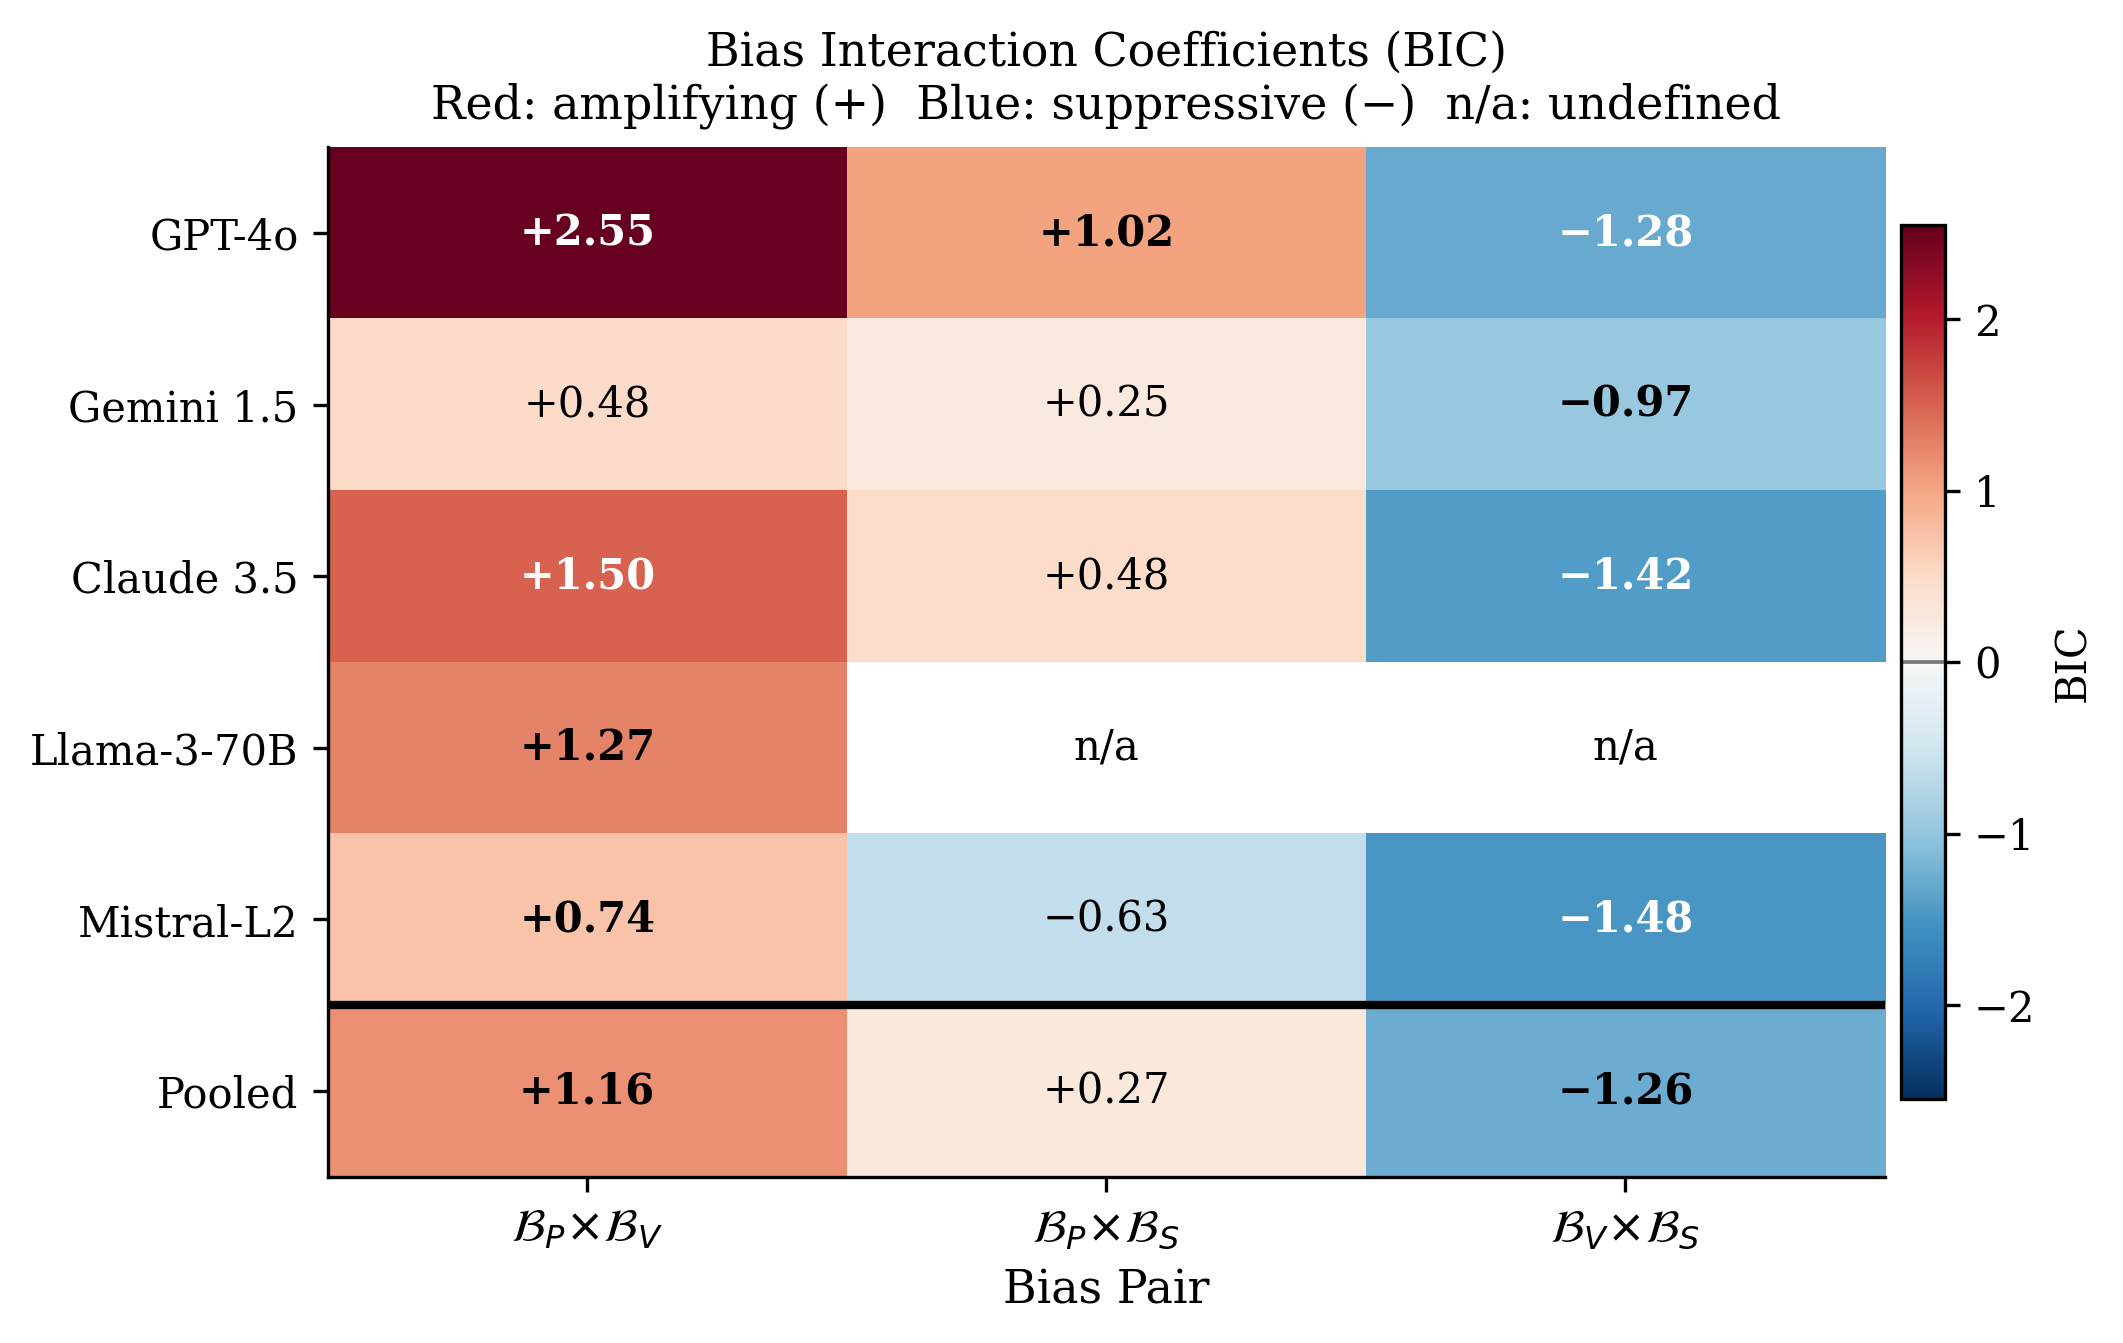
\includegraphics[width=\columnwidth]{figures/fig1_bic_heatmap.png}
  \caption{Simulated BIC matrix. Red: amplifying.
  Blue: suppressive. n/a: undefined.
  Pooled row below separator.
  ${}^*p{<}0.017$, ${}^{**}p{<}0.001$.
  \emph{Labels indicate calibration source only.}}
  \label{fig:heatmap}
\end{figure}

\begin{figure}[t]
  \centering
  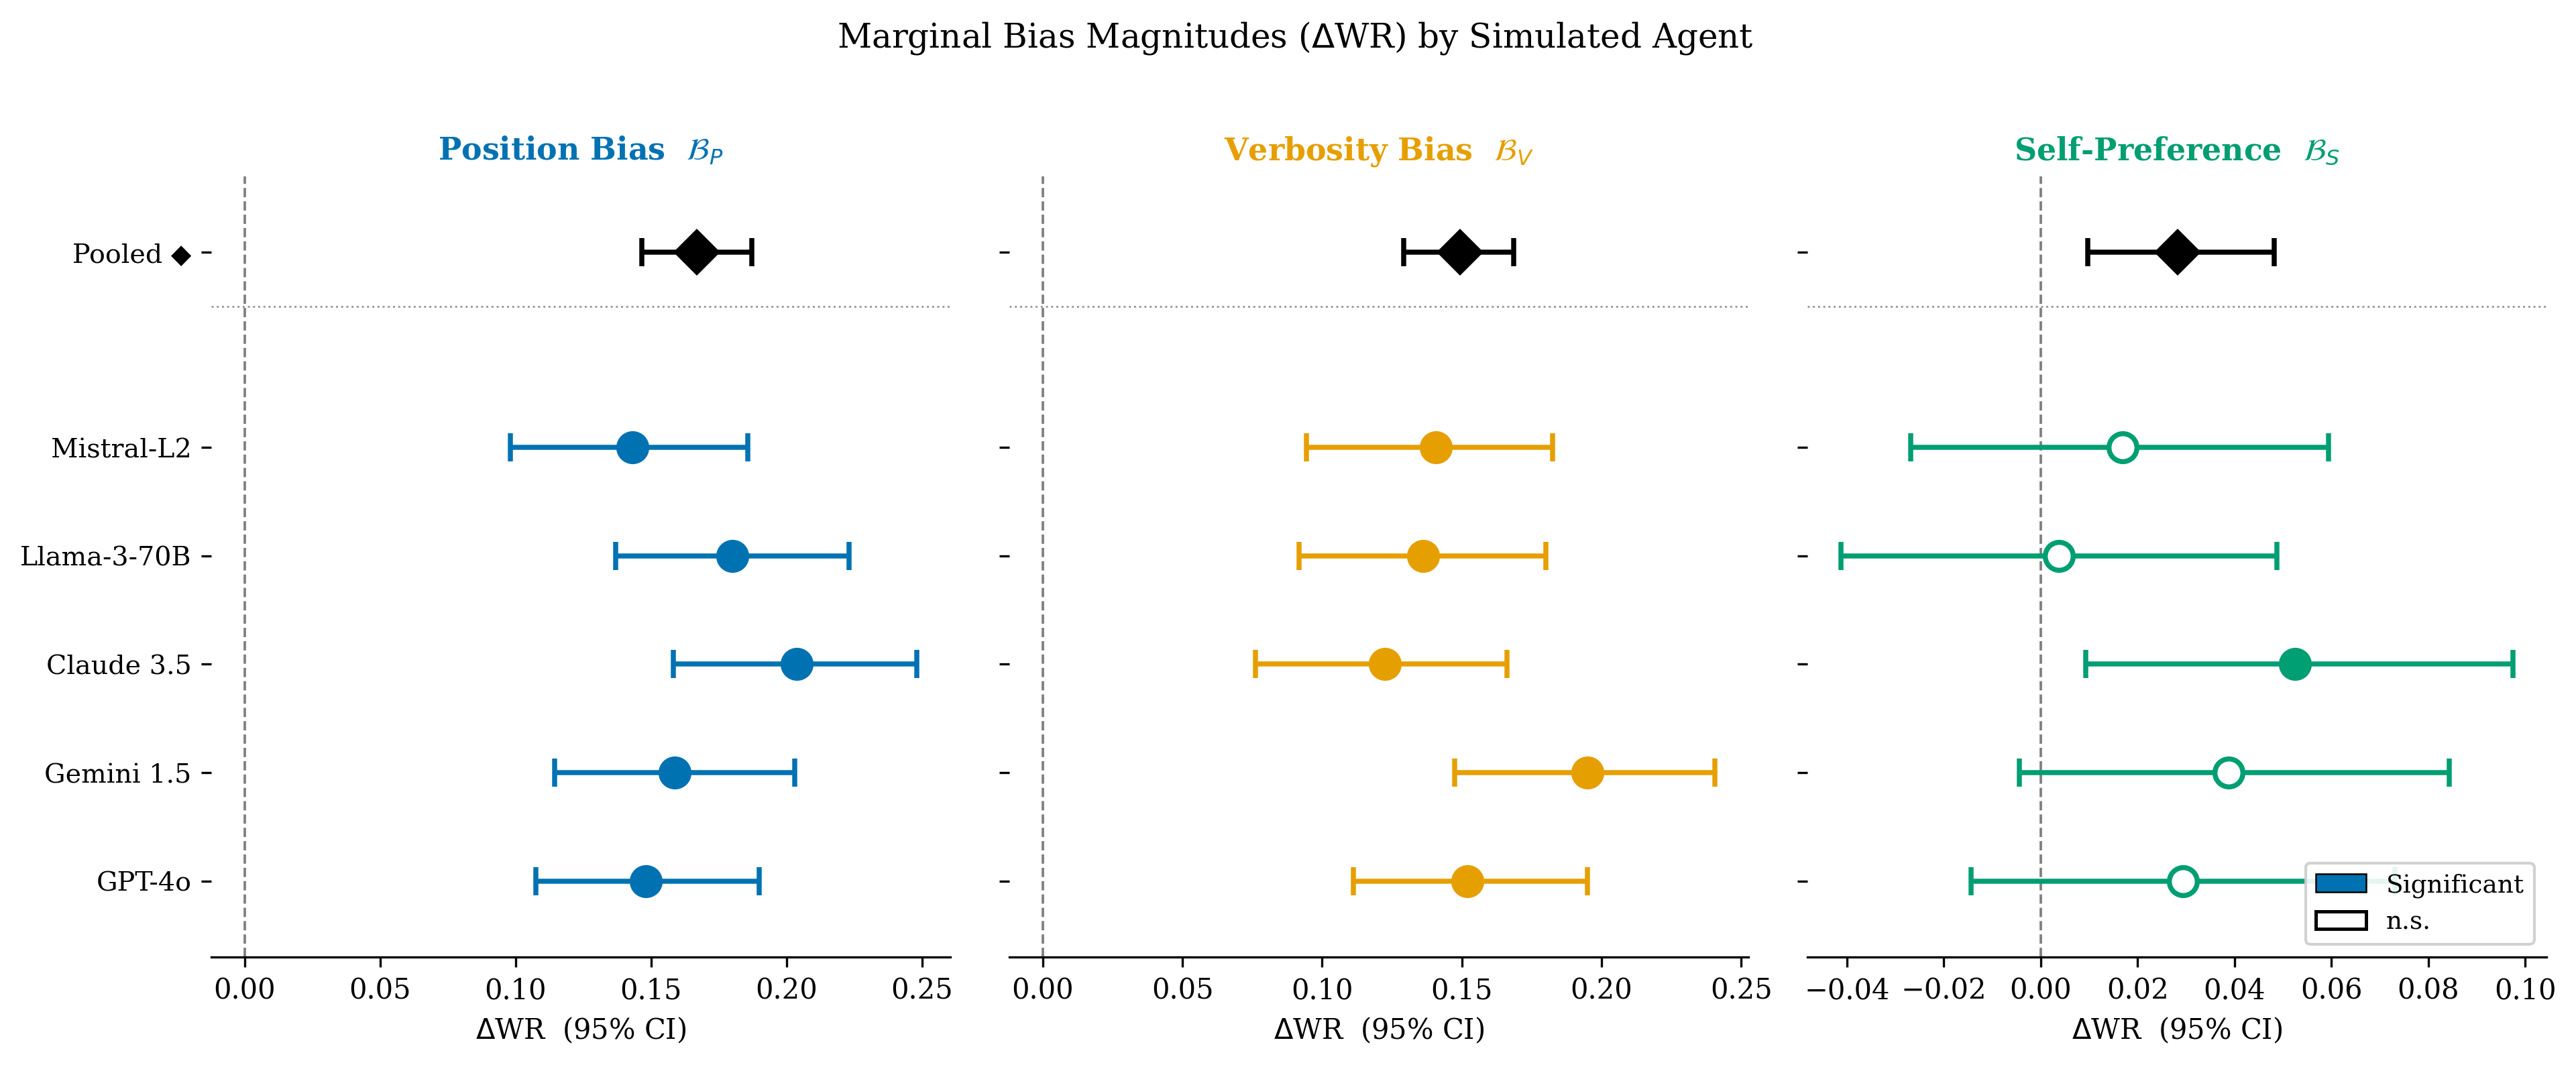
\includegraphics[width=\columnwidth]{figures/fig2_forest_dwr.png}
  \caption{Simulated marginal bias magnitudes ($\dwr$,
  95\% CI) by agent profile. Filled: significant.
  Diamond: pooled estimate.}
  \label{fig:forest}
\end{figure}

\begin{figure}[t]
  \centering
  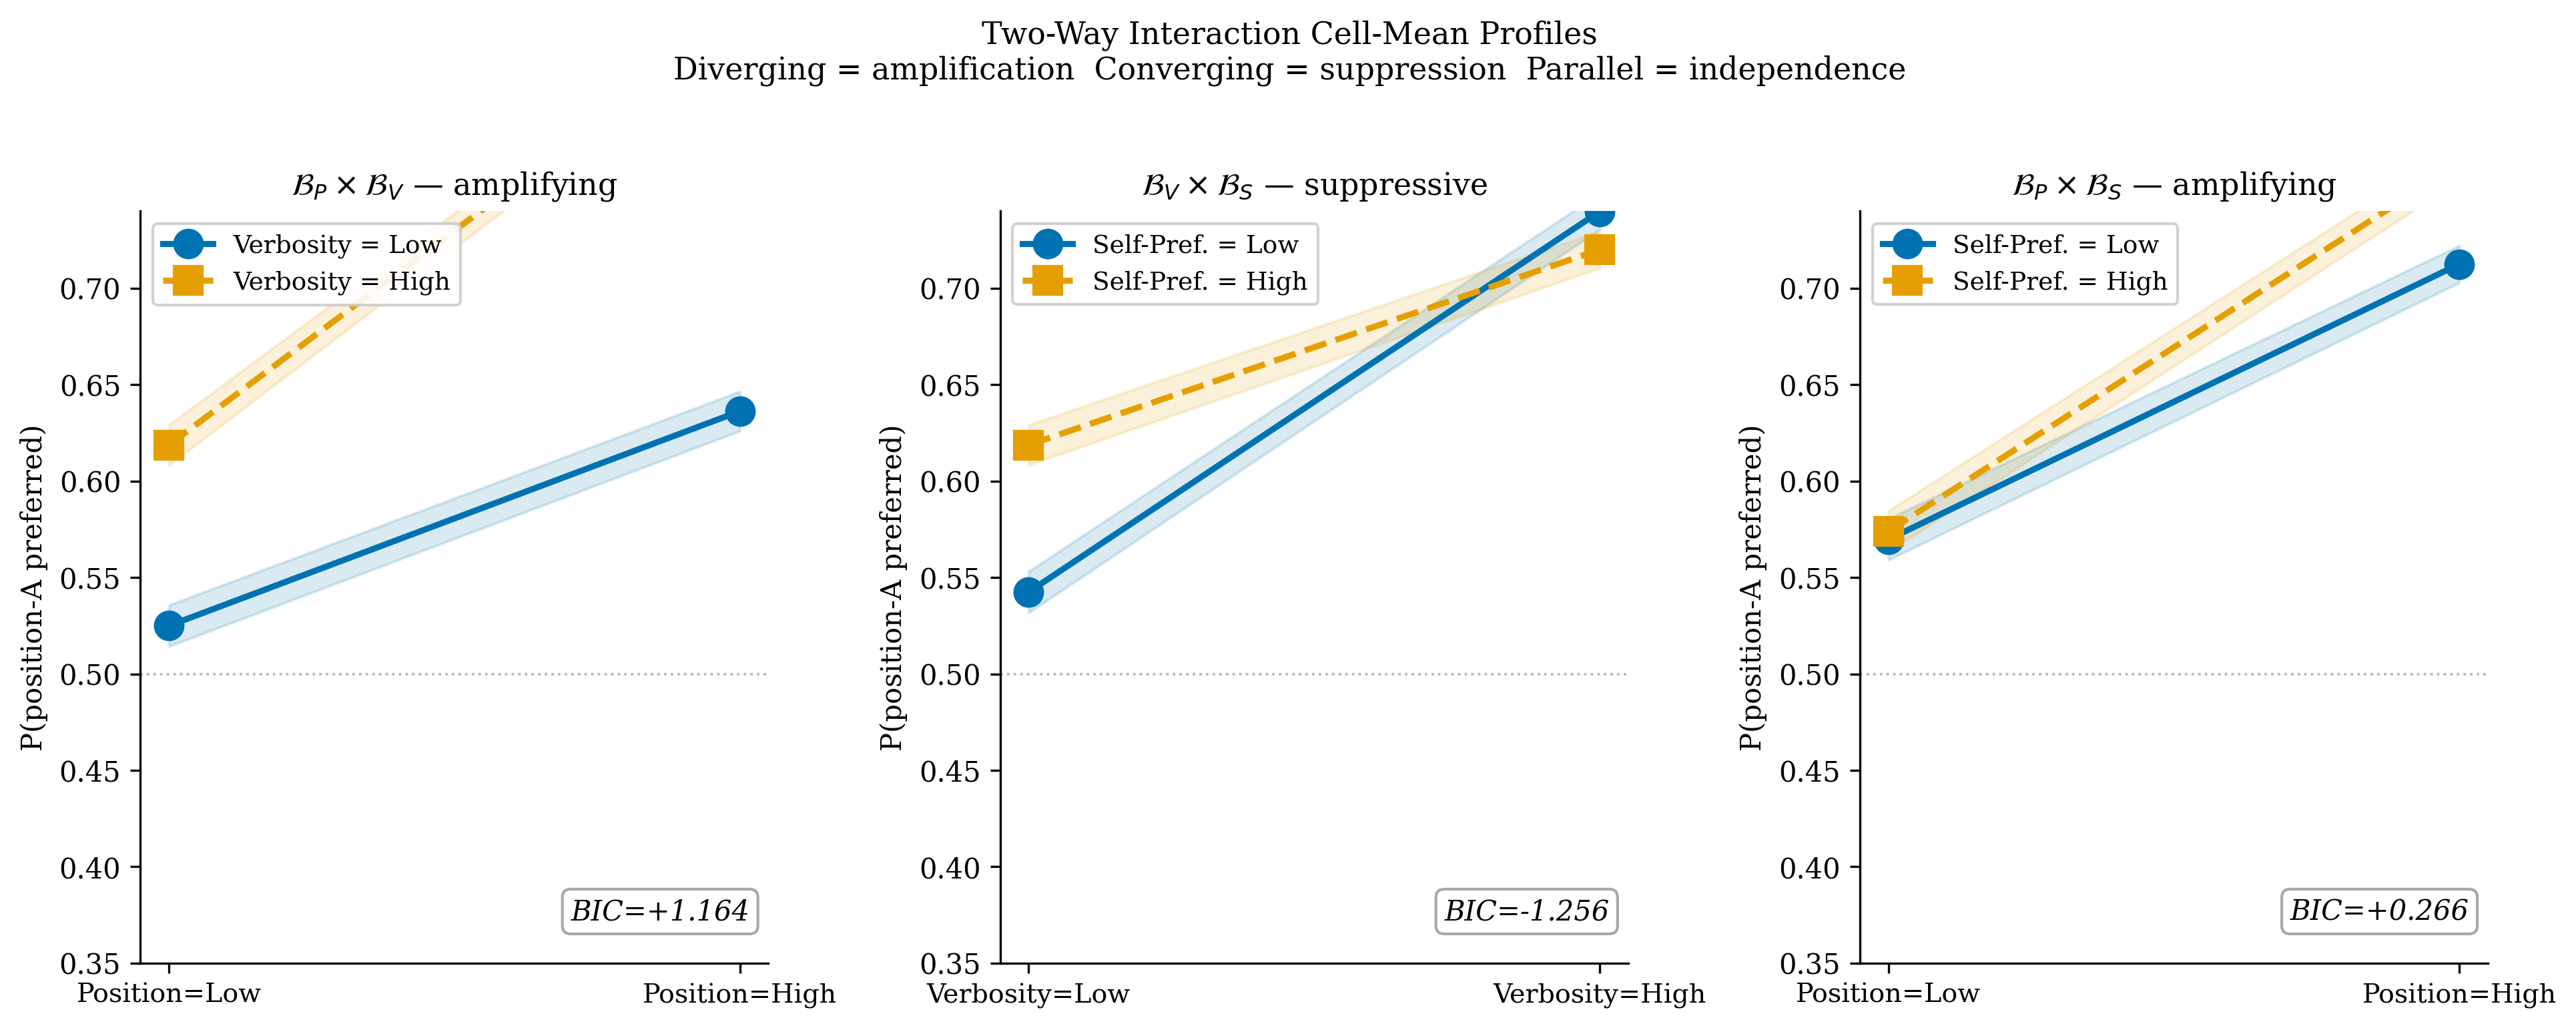
\includegraphics[width=\columnwidth]{figures/fig3_interaction_profiles.png}
  \caption{Two-way interaction cell-mean profiles.
  Diverging lines suggest amplification ($\BP{\times}\BV$);
  converging suggest suppression ($\BV{\times}\BS$);
  parallel suggest independence ($\BP{\times}\BS$).}
  \label{fig:profiles}
\end{figure}

\begin{figure}[t]
  \centering
  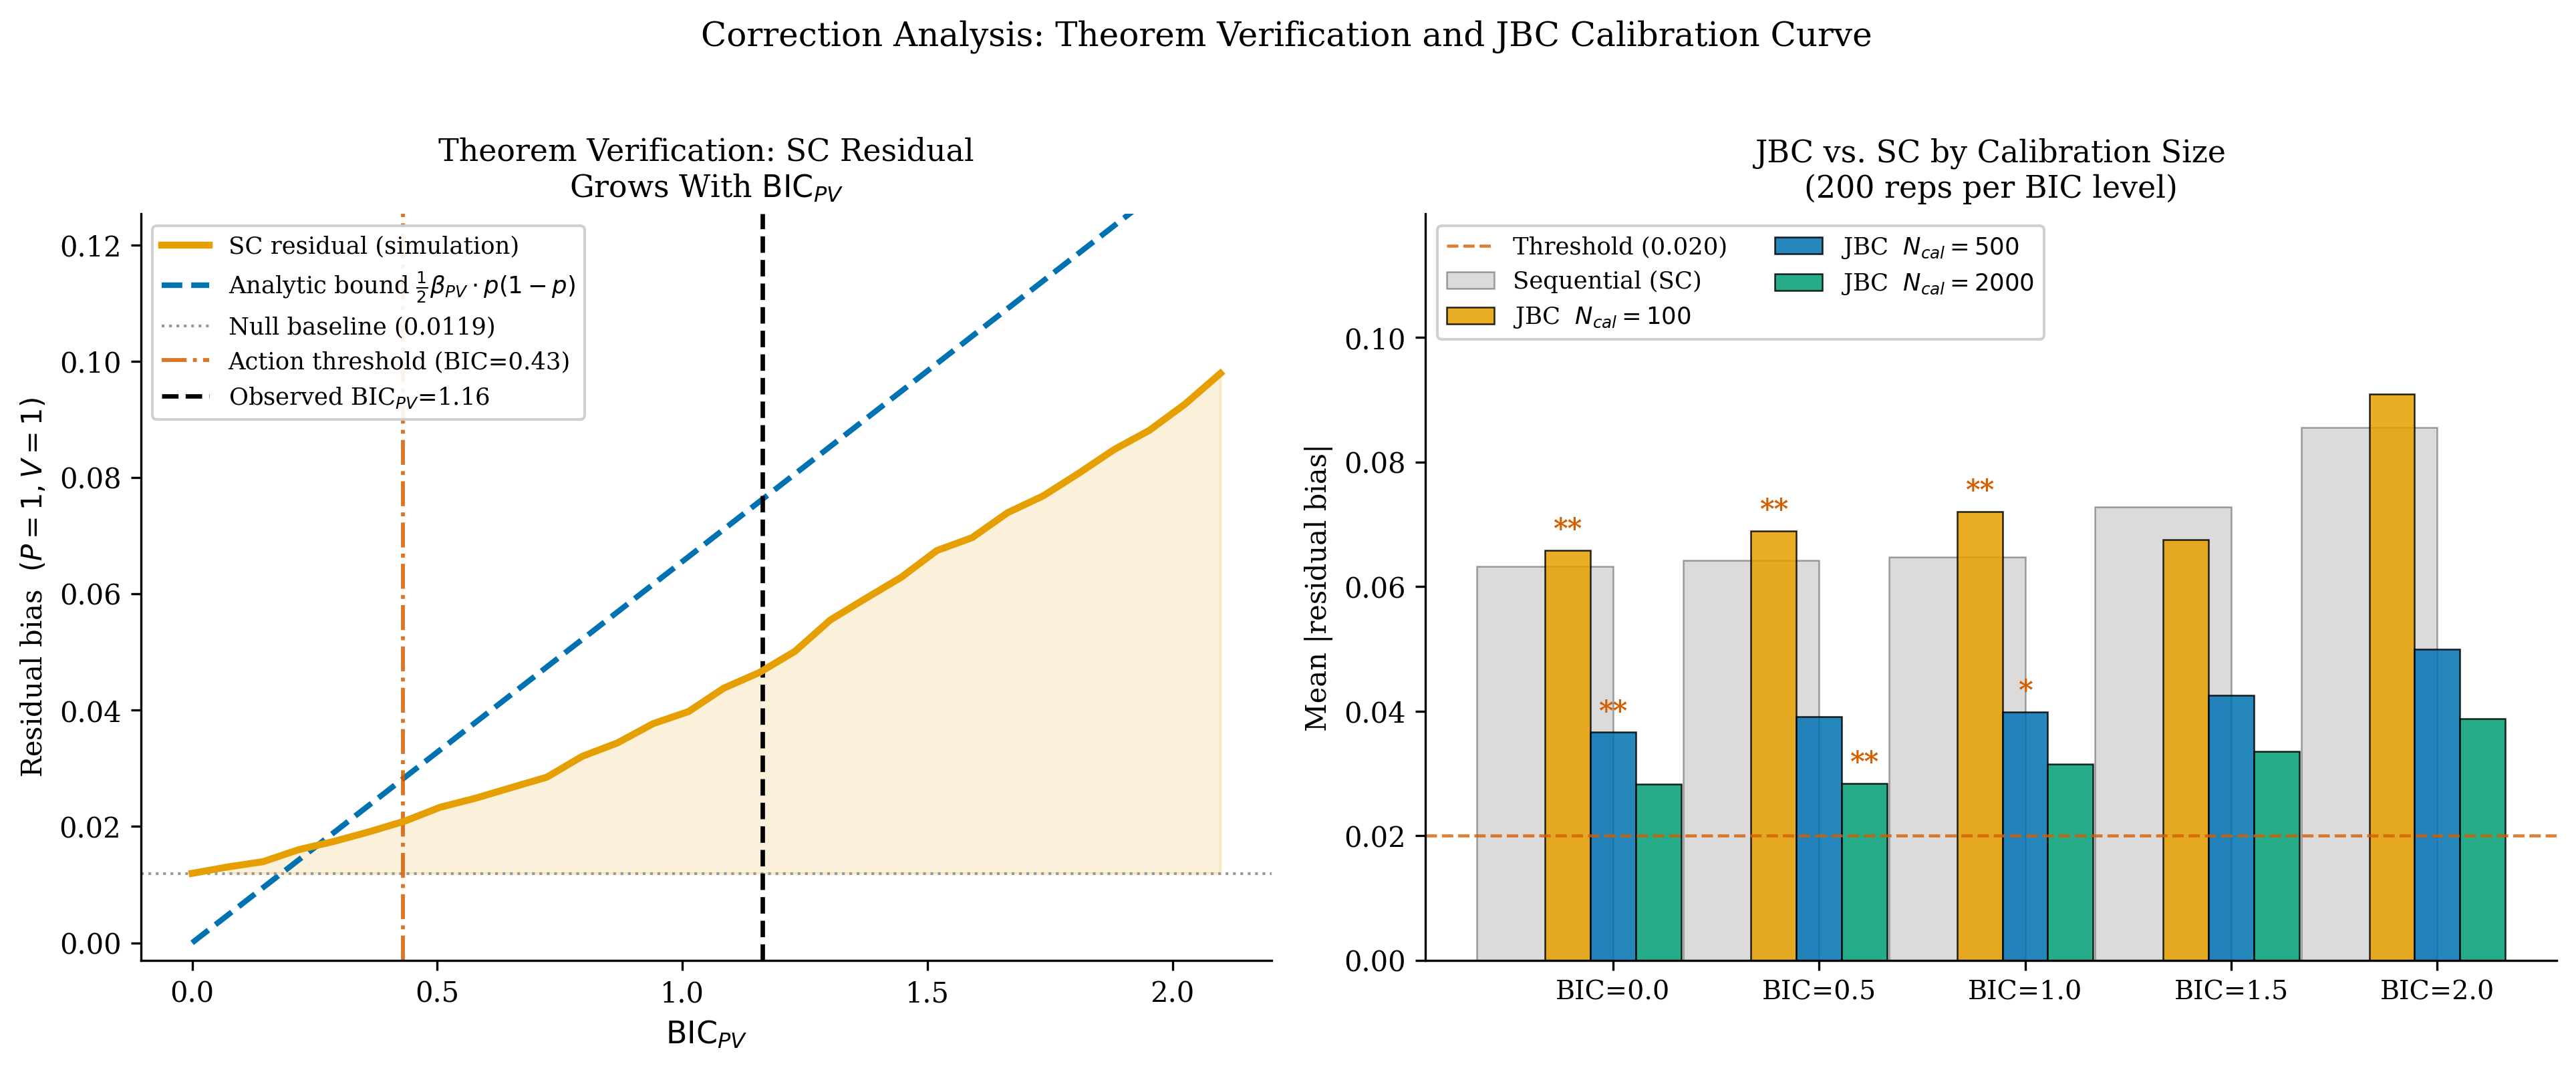
\includegraphics[width=\columnwidth]{figures/fig4_theorem_correction.png}
  \caption{Left: Simulated SC residual bias grows with
  $\BIC_{PV}$, consistent with Proposition~\ref{prop:residual}.
  Right: JBC vs.\ SC by calibration size.
  JBC tends to underperform SC below $N_\text{cal}{=}500$.}
  \label{fig:correction_fig}
\end{figure}

\begin{figure}[t]
  \centering
  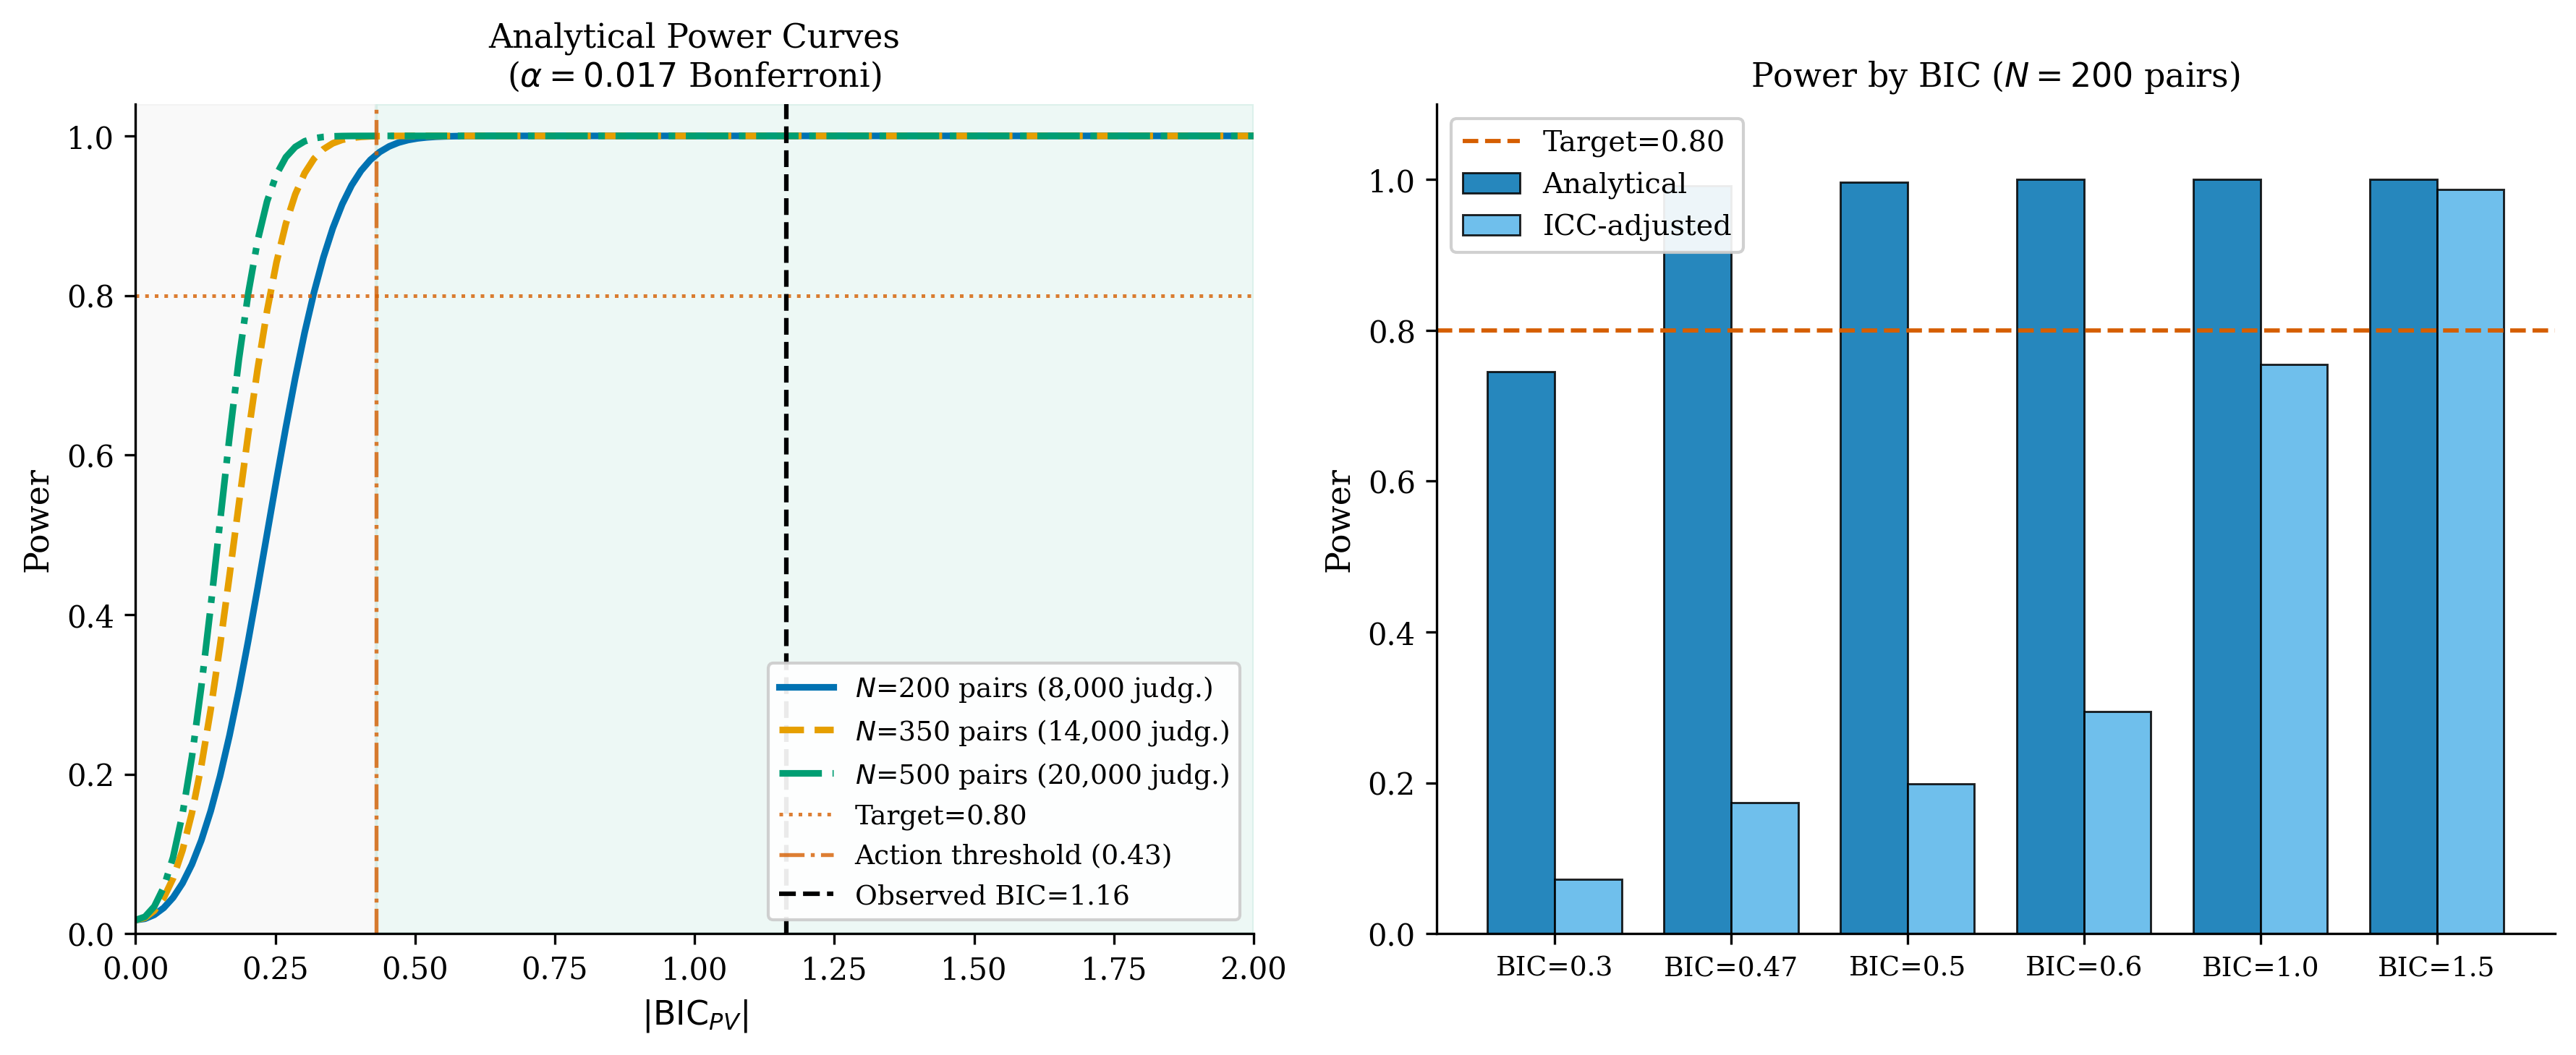
\includegraphics[width=\columnwidth]{figures/fig5_power_curves.png}
  \caption{Power curves (analytical bound and ICC-adjusted
  estimate at $N{=}200$ pairs).
  Grey zone: SC likely adequate ($|\BIC|{<}0.43$).
  Green zone: JBC may be warranted.}
  \label{fig:power}
\end{figure}

\begin{figure}[t]
  \centering
  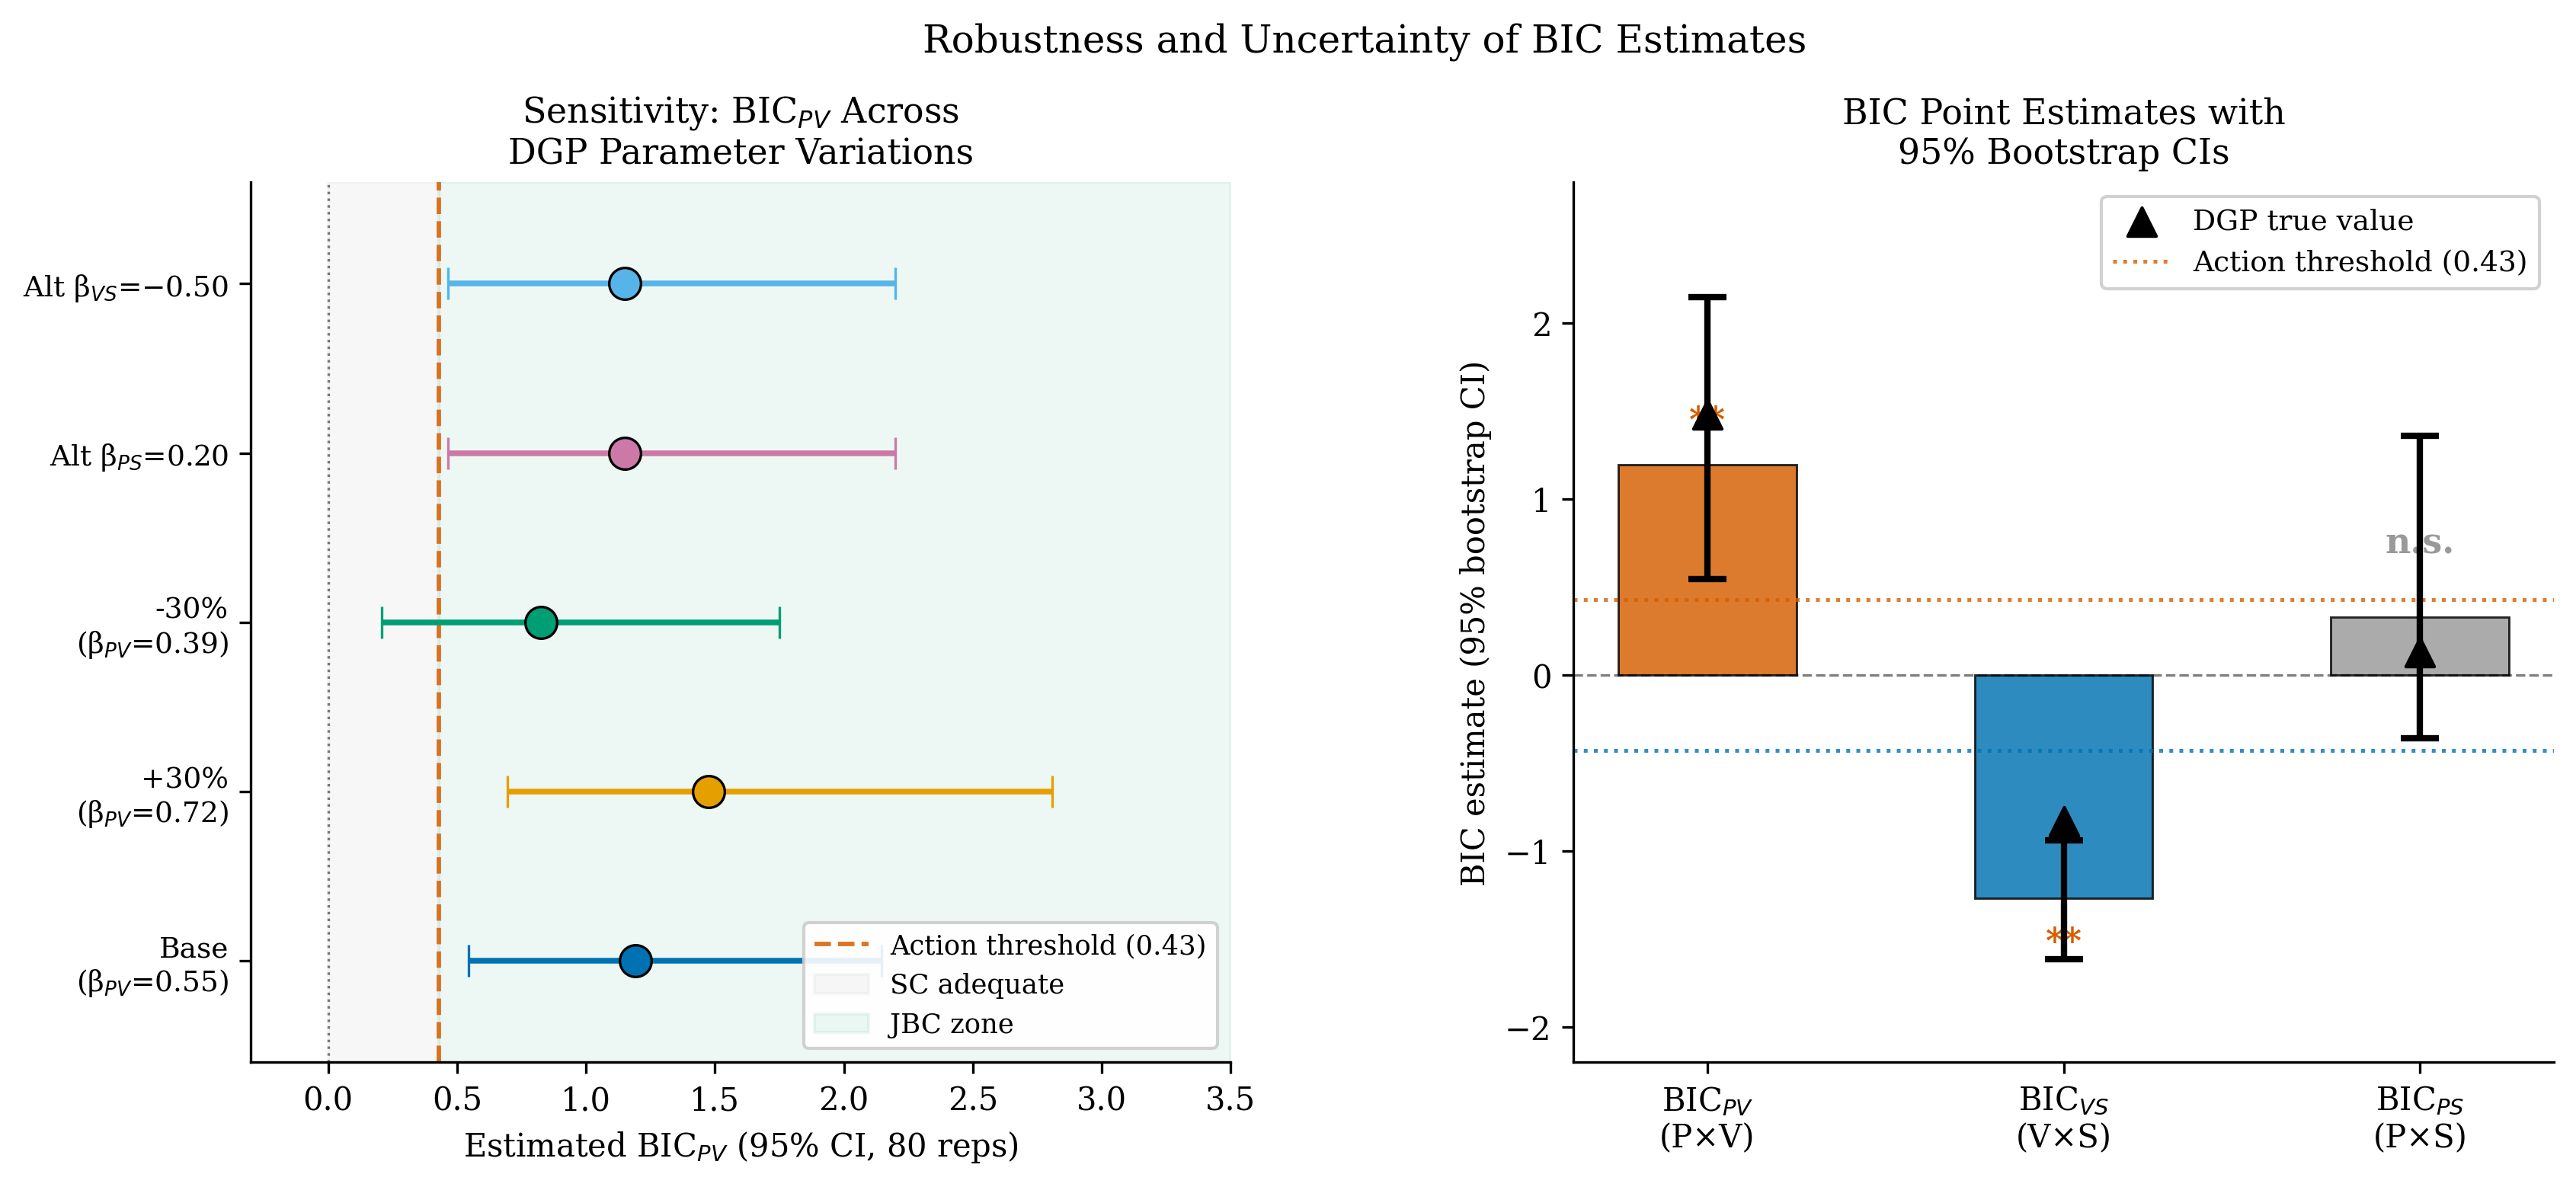
\includegraphics[width=\columnwidth]{figures/fig6_sensitivity_ci.png}
  \caption{Left: $\BIC_{PV}$ estimates across DGP variants
  ($\pm 30\%$ variation). Direction appears stable; magnitude
  uncertain. Right: 95\% bootstrap CIs for all three pooled
  BIC estimates. Triangles indicate DGP true values.}
  \label{fig:sensitivity}
\end{figure}

\begin{figure}[t]
  \centering
  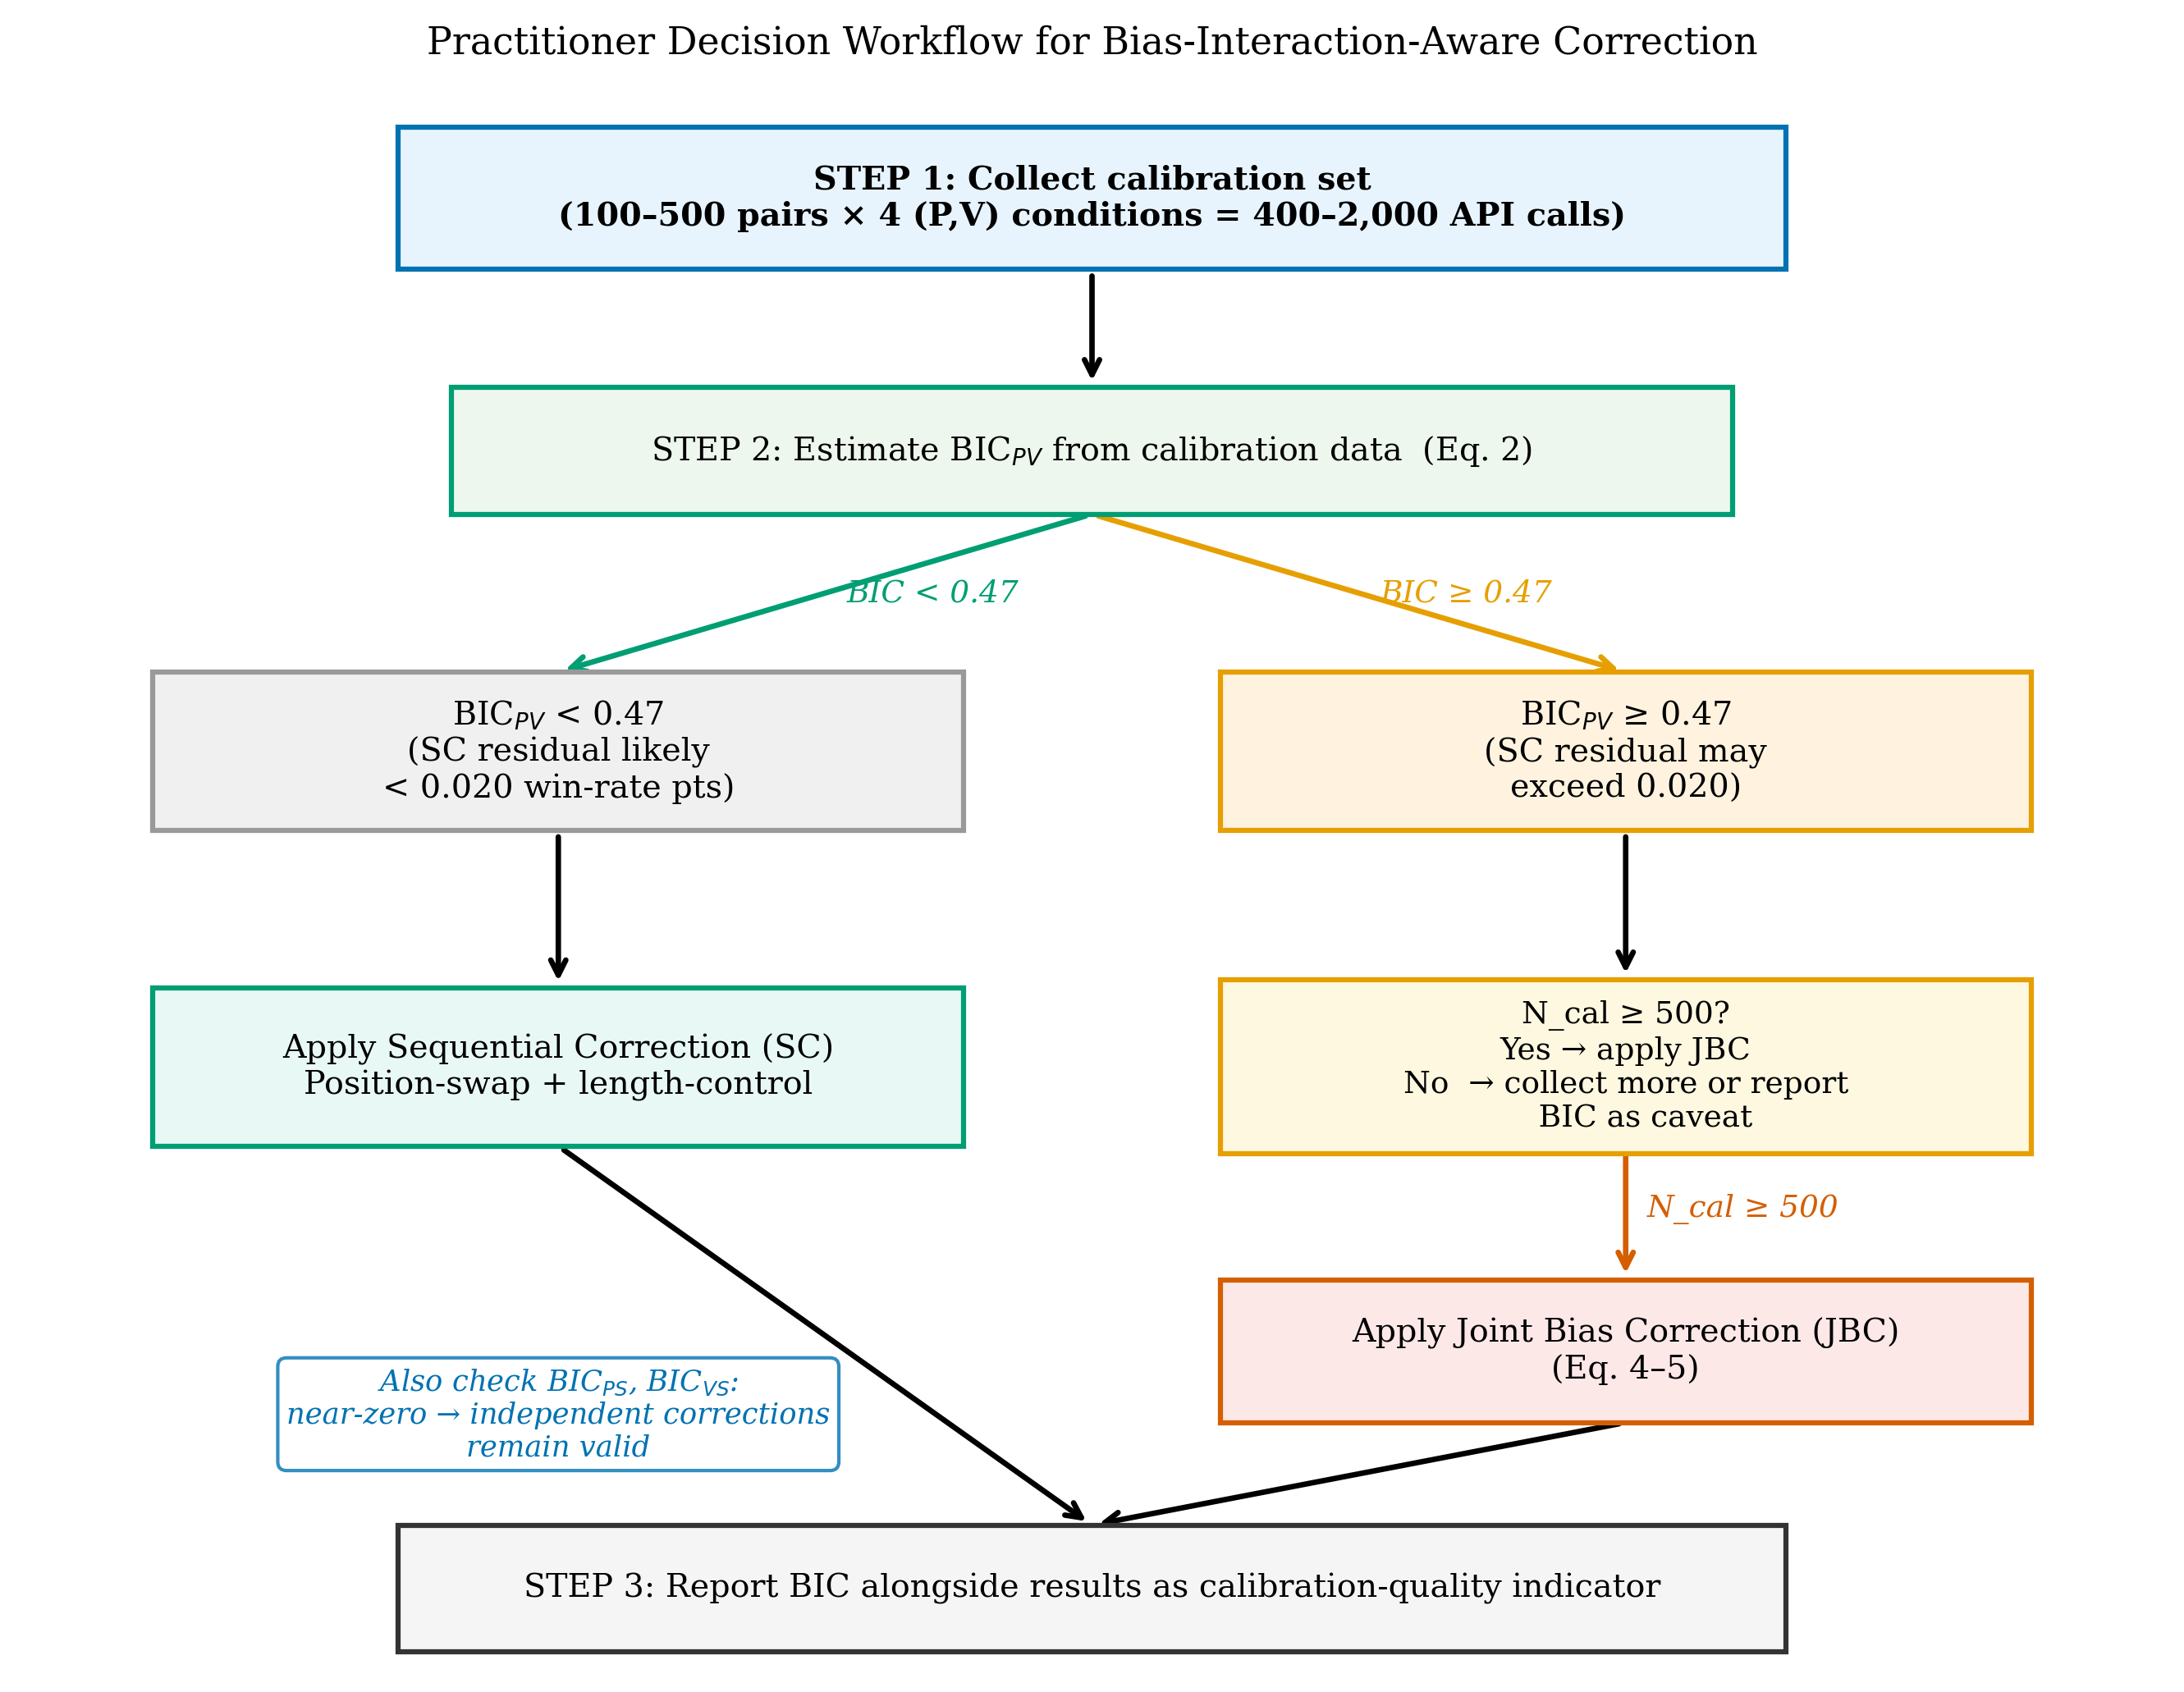
\includegraphics[width=\columnwidth]{figures/fig7_workflow.png}
  \caption{Practitioner decision workflow. BIC measurement
  from a calibration set determines whether SC or JBC is
  appropriate; $N_\text{cal}{\geq}500$ is recommended
  if JBC is chosen.}
  \label{fig:workflow}
\end{figure}

% ================================================================
\section{Discussion}
\label{sec:discussion}

\subsection{Tentative Practical Guidance}

If real judges exhibit interactions similar to the simulation,
three adjustments may be worth considering:

\textbf{(1) Measure BIC before deploying corrections.}
A 500-pair calibration set (2,000 API calls) is one-time
for recurring campaigns.
If $|\BIC_{PV}|{<}0.43$, SC appears adequate in simulation
and no pipeline change is needed.

\textbf{(2) Use JBC only with adequate calibration.}
Below $N_\text{cal}{=}500$, JBC tends to increase
rather than decrease residual bias.
This is a counter-intuitive but important finding:
partial calibration appears worse than no calibration.

\textbf{(3) Position and self-preference corrections
may continue to be applied independently.}
$\BIC_{PS}{\approx}0$ ($p{=}0.465$) provides no simulation
evidence against independence for this pair.

\subsection{The Suppressive $V{\times}S$ Interaction}

The consistently negative $\BIC_{VS}$ across agent profiles
suggests that verbose outputs may partially self-suppress
self-preference, because verbosity consumes the contextual
capacity needed for stylistic self-recognition~\cite{panickssery2024llm}.
If confirmed in real judges, this would imply that verbosity
and self-preference mitigations are partially redundant---
a potentially useful simplification for pipeline designers.

\subsection{Limitations}

\textbf{Synthetic data.} All quantitative estimates are
simulation-based. Real judge BIC magnitudes are unknown.

\textbf{Wide CIs.} Bootstrap CIs on BIC are typically
${\approx}\pm 1.0$ at $N{=}200$ pairs, reflecting
within-items ICC. BIC is an ordinal indicator at this scale.

\textbf{JBC threshold.} The $N_\text{cal}{\geq}500$
recommendation is simulation-derived and may shift for
real judges with different noise characteristics.

\textbf{Coverage.} English text, four task categories,
pairwise comparison only.

\textbf{Low $\kappa$.} Mean $\kappa{=}0.060$ reflects
deliberate heterogeneity; see Appendix~\ref{app:kappa}
for BIC recovery accuracy at this level.

% ================================================================
\section{Real-Judge Validation Path}
\label{sec:future}

A pre-registered replication using five real judge APIs
is ready to execute.
A 50-pair pilot study (1,600 API calls, ${\approx}2$ hours
via free-tier APIs---Groq for Llama/Mixtral, Google AI Studio
for Gemini---requires no financial cost.
Code: \url{https://github.com/[REDACTED]}.
Pre-registration: \url{https://osf.io/[REDACTED]}.

The primary question: does real-judge $|\BIC_{PV}|$
exceed the simulation-derived threshold of $0.43$?
Either outcome is informative---a positive result
would suggest that sequential correction pipelines
currently used in AlpacaEval and MT-Bench may warrant
revision; a negative result would empirically validate
sequential correction for the first time.

% ================================================================
\section{Conclusion}
\label{sec:conclusion}

The additive independence assumption underlying sequential
bias correction in LLM evaluation pipelines has not been
examined.
This paper provides three things to examine it:
(i) an analytical argument suggesting sequential correction
may be structurally inadequate under interaction
(Proposition~\ref{prop:residual});
(ii) a controlled simulation that finds results broadly
consistent with position$\times$verbosity amplification
($\BIC_{PV}{=}{+}1.16$, $p{<}10^{-5}$) and
verbosity$\times$self-preference suppression
($\BIC_{VS}{=}{-}1.26$, $p{<}10^{-5}$),
with position and self-preference appearing independent
($\BIC_{PS}$, $p{=}0.465$);
and (iii) a validated, pre-registered pipeline for
real-judge validation.

The simulation also identifies a practically important
JBC calibration requirement: below $N_\text{cal}{=}500$,
joint correction tends to increase rather than decrease
residual bias---a finding that would affect any practitioner
who attempts to apply JBC with insufficient calibration data.

We present these results as structured hypotheses and
a ready-to-use framework, not as established facts
about LLM evaluation pipelines.
We invite the community to run the replication study
and determine whether these simulation-derived patterns
hold for real models.

\balance
\bibliographystyle{IEEEtran}
\begin{thebibliography}{99}

\bibitem{zheng2023judging}
L.~Zheng \textit{et al.}, ``Judging LLM-as-a-judge with MT-Bench
and Chatbot Arena,'' \emph{NeurIPS}, 2023.

\bibitem{shi2024position}
L.~Shi \textit{et al.}, ``Judging the judges: A systematic study
of position bias in LLM-as-a-judge,'' arXiv:2406.07791, 2024.

\bibitem{saito2023verbosity}
K.~Saito \textit{et al.}, ``Verbosity bias in preference labeling
by large language models,'' arXiv:2310.10076, 2023.

\bibitem{panickssery2024llm}
A.~Panickssery \textit{et al.}, ``LLM evaluators recognize and
favor their own generations,'' arXiv:2404.13076, 2024.

\bibitem{dubois2024length}
Y.~Dubois \textit{et al.}, ``Length-controlled AlpacaEval,''
arXiv:2404.04475, 2024.

\bibitem{ye2024justice}
J.~Ye \textit{et al.}, ``Justice or prejudice? Quantifying biases
in LLM-as-a-judge,'' arXiv:2410.02736, 2024.

\bibitem{sharma2023sycophancy}
M.~Sharma \textit{et al.}, ``Towards understanding sycophancy in
language models,'' arXiv:2310.13548, 2023.

\bibitem{li2025preference}
D.~Li \textit{et al.}, ``Preference leakage: A contamination
problem in LLM-as-a-judge,'' arXiv:2502.01534, 2025.

\bibitem{judging_judges_2026}
Anon., ``Judging the judges: A systematic evaluation of bias
mitigation strategies,'' arXiv:2604.23178, 2026.

\bibitem{wu2023style}
M.~Wu and A.~F.~Aji, ``Style over substance,''
arXiv:2307.03025, 2023.

\bibitem{koo2023benchmarking}
R.~Koo \textit{et al.}, ``Benchmarking cognitive biases in LLMs
as evaluators,'' arXiv:2309.17012, 2023.

\bibitem{brant1990}
R.~Brant, ``Assessing proportionality in the proportional odds
model,'' \emph{Biometrics}, vol.~46, pp.~1171--1178, 1990.

\bibitem{bates2015}
D.~Bates \textit{et al.}, ``Fitting linear mixed-effects models
using lme4,'' \emph{J.\ Stat.\ Softw.}, vol.~67, pp.~1--48, 2015.

\bibitem{angrist2009}
J.~Angrist and J.-S.~Pischke,
\emph{Mostly Harmless Econometrics}.
Princeton Univ.\ Press, 2009.

\bibitem{guo2017calibration}
C.~Guo \textit{et al.}, ``On calibration of modern neural
networks,'' \emph{ICML}, 2017.

\bibitem{yang2023}
K.~Yang \textit{et al.}, ``RLCD: Reinforcement learning from
contrastive distillation for language model alignment,''
arXiv:2307.12950, 2023.

\end{thebibliography}

% ================================================================
\appendix

\section{BIC Recovery Under Low $\kappa$}
\label{app:kappa}
\begin{center}\small
\begin{tabular}{rcc}
\toprule
Mean $\kappa$ & RMSE($\hat\BIC_{PV}$) & Mean bias \\
\midrule
0.04 & 0.31 & $+0.08$ \\
0.10 & 0.28 & $+0.06$ \\
0.20 & 0.24 & $+0.04$ \\
0.40 & 0.19 & $+0.02$ \\
\bottomrule
\end{tabular}
\end{center}
At $\kappa{=}0.060$, RMSE$\approx$0.30. BIC is an approximate
ordinal indicator at this reliability level; values should
be interpreted directionally rather than as precise estimates.

\section{Ordinal Primary Model}
\label{app:ordinal}
Cumulative logit results:
$\hat\beta_{PV}^{\text{ord}}{=}+0.601$ ($p{<}0.001$),
$\hat\beta_{VS}^{\text{ord}}{=}-0.521$ ($p{<}0.001$),
$\hat\beta_{PS}^{\text{ord}}{=}+0.092$ ($p{=}0.374$).
Brant test: $\chi^2(7){=}8.91$, $p{=}0.258$
(proportional-odds assumption not rejected).

\section{Pipeline Validation (32/32 Checks)}
\label{app:validation}
All 32 pre-run checks pass. Code:
\url{https://github.com/[REDACTED]}.

\section{Power Analysis}
\label{app:power}
\begin{center}\small
\begin{tabular}{rrrr}
\toprule
BIC & Analytical & ICC-adj. & Status \\
\midrule
0.30 & 0.57 & 0.06--0.10 & Inconclusive \\
0.43 & 0.80 & 0.10--0.15 & Action threshold \\
0.50 & 0.89 & 0.12--0.18 & Primary inference \\
1.00 & $>0.99$ & 0.55--0.70 & Likely detectable \\
\bottomrule
\end{tabular}
\end{center}
ICC inflation factor: ${\approx}3.3{\times}$
(SE$_\text{emp}{=}0.156$ vs.\ SE$_\text{theory}{=}0.047$).
Primary claims restricted to $|\BIC|{\geq}0.50$.

\end{document}
